\documentclass{article}
%\usepackage[english]{babel}%
\usepackage{graphicx}
\usepackage{tabulary}
\usepackage{tabularx}
\usepackage[table,xcdraw]{xcolor}
\usepackage{pdflscape}
%\usepackage{gensymb}
\usepackage{lastpage}
\usepackage{multirow}
\usepackage{xcolor}
\usepackage{cancel}
\usepackage{amsmath}
\usepackage[table]{xcolor}
\usepackage{fixltx2e}
\usepackage[T1]{fontenc}
\usepackage[utf8]{inputenc}
\usepackage{ifthen}
\usepackage{fancyhdr}
\usepackage[utf8]{inputenc}
\usepackage{tikz}
\usepackage[document]{ragged2e}
\usepackage[margin=1in,top=1.2in,headheight=57pt,headsep=0.1in]
{geometry}
\usepackage{ifthen}
\usepackage{fancyhdr}
\everymath{\displaystyle}
\usepackage[document]{ragged2e}
\usepackage{fancyhdr}
\usepackage{mathabx}
\usepackage{textcomp,mathcomp}
\usepackage[shortlabels]{enumitem}
\everymath{\displaystyle}
\linespread{2}%controls the spacing between lines. Bigger fractions means crowded lines%
\linespread{1.3}%controls the spacing between lines. Bigger fractions means crowded lines%
\pagestyle{fancy}
\setlength{\headheight}{56.2pt}
\usepackage{soul}
\usepackage{siunitx}

%\usepackage{textcomp}
\usetikzlibrary{shapes.multipart, shapes.geometric, arrows}
\usetikzlibrary{calc, decorations.markings}
\usetikzlibrary{arrows.meta}
\usetikzlibrary{shapes,snakes}
\usetikzlibrary{quotes,angles, positioning}
%\chead{\ifthenelse{\value{page}=1}{
\includegraphics[scale=0.3]{BassettCTCLogo}}}
%\rhead{\ifthenelse{\value{page}=1}{Final Exam}{}}
%\lhead{\ifthenelse{\value{page}=1}{Water Treatment - Oct-Dec 2022}{\textbf Final Exam}}
%\rfoot{\ifthenelse{\value{page}=1}{}{}}
%
%\cfoot{}
%\lfoot{Page \thepage\ of \pageref{LastPage}}
%\renewcommand{\headrulewidth}{2pt}
%\renewcommand{\footrulewidth}{1pt}
\graphicspath{ {./images/} }
\begin{document}
\begin{enumerate}

      \item Water is moving through a 10 inch pipe at a rate of 4.2 feet per second. What is the flow?\\
a) $3.51 \mathrm{cuft} / \mathrm{sec}$\\
b) $7.72 \mathrm{cuft} / \mathrm{sec}$\\
c) $5.61 \mathrm{cuft} / \mathrm{sec}$\\
*d) $2.28 \mathrm{cuft} / \mathrm{sec}$\\

      \item Water if flowing through a completely filled 10 inch line at 4 cuft/sec. What is the velocity?\\
a) $.4 \mathrm{fps}$\\
*b) $7.3 \mathrm{fps}$\\
c) $2.5 \mathrm{fps}$\\
d) $4.0 \mathrm{cuft} / \mathrm{sec}$\\

  \item Water is moving through a 22 inch pipe at a velocity of $3.5 \mathrm{fps}$. What is the flow?\\
a) $6.77 \mathrm{cuft} / \mathrm{sec}$\\
b) $.15 \mathrm{cuft} / \mathrm{sec}$\\
c) $4.6 \mathrm{fps}$\\
*d) $9.2 \mathrm{cuft} / \mathrm{sec}$\\

  \item The flow of a 48 inch pipe is $8590 \mathrm{gpm}$. What is the velocity?\\
a) $3.05 \mathrm{fps}$\\
b) $4.77 \mathrm{fps}$\\
*c) $1.52 \mathrm{fps}$\\
d) $2.33 \mathrm{fps}$\\

\item Calculate the flow velocity in feet/minute if 7.5 MGD of flow passes through a channel that is 3' wide x 4' deep, and the depth of flow is 15 inches.
\begin{center}
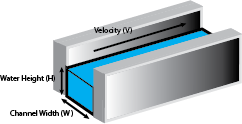
\includegraphics[scale=1.1]{ChannelFlow1}
\end{center}
$Flow (Q) = Velocity (V) * Area (A)$\\
\vspace{0.3cm}
$\implies 7.5 \frac{MG}{day}* \frac{10^6 gal}{MG} * \frac{ft^3}{7.48 gal}*\frac{day}{24*60} \dfrac{ft^3}{min} = V \frac{ft}{min}* 3 ft * \frac{15}{12} ft$\\
\vspace{0.3cm}
$\implies V \frac{ft}{min}= \frac{7.5* 10^6}{7.48*24*60}\frac{ft^3}{min}*\dfrac{1}{\dfrac{3*15\enspace ft^2}{12}}= \boxed{186\frac{ft}{min}}$\\
\vspace {8mm}

\item Calculate the velocity of a 14 MGD flow in a 6 ft wide channel with a water depth of two feet. (5 points)\\
\begin{center}
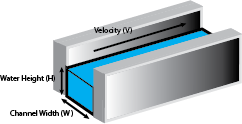
\includegraphics[scale=1.1]{ChannelFlow1}
\end{center}
$Flow (Q) = Velocity (V) * Area (A)$\\
\vspace{0.3cm}
$\implies 14 \frac{MG}{day}* \frac{10^6 gal}{MG} * \frac{ft^3}{7.48 gal}*\frac{day}{24*60*60} = V \frac{ft}{sec}* 6 ft * 2 ft = 12Vft^3$\\
\vspace{0.3cm}
$\implies V \frac{ft}{sec}= \frac{14 * 10^6}{7.48 *12*24*60*60}= \boxed{1.8\frac{ft}{sec}}$\\
\vspace {8mm}

\item A plastic float takes 9.8 seconds to travel a distance of 25 feet in a channel. The channel is 3 ft 8 in. wide and the water level in this channel is 28 inches. What is the flow in GPM\\
Solution:\\
\vspace{0.3cm}
$Q=V*A$\\
\vspace{0.3cm}
$\implies Q=\dfrac{25ft}{9.8s}*\Big((3+\dfrac{8}{12})*\dfrac{28}{12}\Big)ft^2*7.48\dfrac{gal}{ft^3}*60\dfrac{s}{min}=\boxed{9,795\dfrac{gal}{min}}$



\item Calculate the flow, in gpd, that would pass through a grit chamber 2 feet wide, at a depth of 6 inches, with a velocity of 1 ft /sec\\
a. 646,272gpd \\
b. 610,000gpd \\
c. 300,272gpd \\
d. 576,534gpd \\
Solution:\\
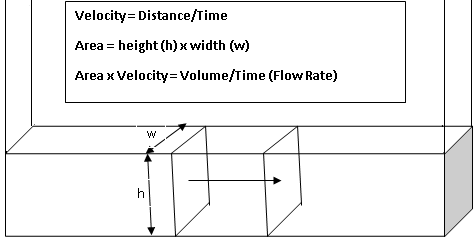
\includegraphics[scale=0.5]{ChannelFlow3}\\
$Q=V*A$\\
\vspace{0.3cm}
$Q=1\dfrac{ft}{s}*(2*0.5)ft^2=1\dfrac{ft^3}{s}$\\
\vspace{0.3cm}
$Q=1\dfrac{\cancel{ft^3}}{\cancel{s}}*\dfrac{(1440*60)\cancel{s}}{day}*7.48\dfrac{gal}{\cancel{ft^3}}=\boxed{646,272\dfrac{gal}{day}}$


\item A channel is 3.25 feet wide and is conveying a a flow of 3.5 MGD. The depth of the water is 8 inches. Calculate the velocity of this flow.\\
Solution:\\
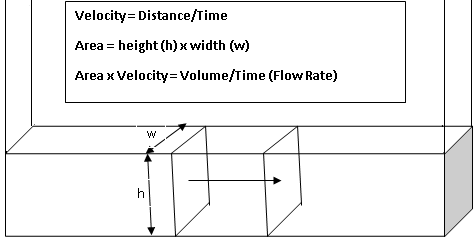
\includegraphics[scale=0.5]{ChannelFlow3}\\
$Q=V*A \implies V=\dfrac{Q}{A}$\\
\vspace{0.3cm}
$\implies V\dfrac{ft}{s}=\dfrac{3.5\dfrac{\cancel{MG}}{\cancel{day}}*\dfrac{1000000\cancel{gal}}{\cancel{MG}}*\dfrac{ft^{\cancel{3}}}{7.48\cancel{gal}}*\dfrac{\cancel{day}}{(1440*60)s}}{(3.25*0.75)\cancel{ft^2}}=\boxed{2.2\dfrac{ft}{s}}$

\item A plastic float is dropped into a channel and is found to travel 10 feet in 4.2 seconds. The channel is 2.4 feet wide and is flowing 1.8 feet deep. Calculate the channel flow rate in cubic feet per second.\\
Solution:\\
$Q=V*A$\\
\vspace{0.3cm}
$\implies Q\Big(\dfrac{ft^3}{s}\Big)=\dfrac{10ft}{4.2s}*(2.4*1.8)ft^2=\boxed{10.3\dfrac{ft^3}{s}}$
\item A 12 inch pipe conveys sewage at 2.6 feet per second.  What is the flow expressed in MGD?
Solution:\\
\vspace{0.3cm}
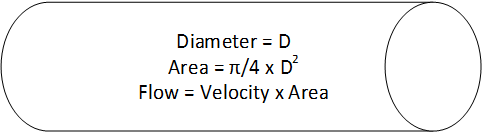
\includegraphics[scale=0.5]{PipeFlow}\\
\vspace{0.3cm}
$Q=V*A$\\
\vspace{0.3cm}
$Q=2.6\dfrac{\cancel{ft}}{\cancel{s}}*0.785*1^2\cancel{ft^2}*7.48\dfrac{\cancel{gal}}{ft^3}*\dfrac{MG}{1,000,000\cancel{gal}}*\dfrac{(1440*60)\cancel{s}}{day}=\boxed{1.3MGD}$\\

\item A line to a water treatment plant is 12 miles long. If the water is flowing at 2.2 fps, how long will it take for water to reach the plant?\\
Solution:\\
$time \enspace to \enspace reach \enspace plant \enspace (hrs)=\dfrac{\cancel{s}}{2.2\cancel{ft}}*\dfrac{5280\cancel{ft}}{\cancel{mile}}*12\cancel{miles}*\dfrac{hrs}{(60*60)\cancel{s}}=\boxed{8hrs}$  



\item A channel is 2 feet 4 inches wide. When water is flowing 8 inches deep in this channel, the flow velocity is found to be 1.6 ft per second. Calculate flow in MGD.\\
\vspace{0.3cm}
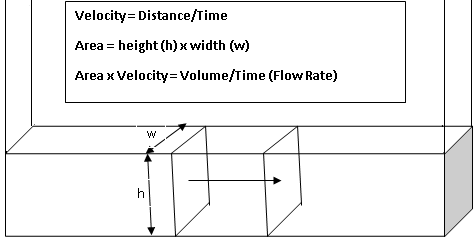
\includegraphics[scale=0.5]{ChannelFlow3}\\
\vspace{0.3cm}
$Q=V*A$\\
\vspace{0.3cm}
$Q=1.6\dfrac{ft}{s}*\Big(\dfrac{28}{12}*\dfrac{8}{12}\Big)ft^2=2.49\dfrac{ft^3}{s}$\\
$Q=2.49\dfrac{\cancel{ft^3}}{\cancel{s}}*\dfrac{(1440*60)\cancel{s}}{day}*7.48\dfrac{\cancel{gal}}{\cancel{ft^3}}\dfrac{MG}{\cancel{gal}}=\boxed{1.61MGD}$


\item What is the velocity (ft/s) of a 3 MGD flow in a 12 in. diameter pipe. Assume the pipe is flowing full.\\
Solution:\\
\vspace{0.3cm}
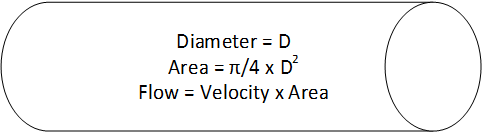
\includegraphics[scale=0.5]{PipeFlow}\\
$Q=V*A$\\
$\implies V=\dfrac{Q}{A} \implies V \Big(\dfrac{ft}{s}\Big)= \dfrac{\dfrac{3\cancel{MG}}{\cancel{day}}*\dfrac{1,000,000\cancel{gal}}{\cancel{MG}}*\dfrac{ft^{\cancel{3}}}{7.48\cancel{gal}}*\dfrac{\cancel{day}}{1440*60s}}{0.785*\Big(\dfrac{12}{12}\Big)^2\cancel{ft^2}}=\boxed{5.9ft/s}$



\item What is the velocity in cfs of 10 mgd flow in a full 24” pipe?
Solution:\\
\vspace{0.5cm}
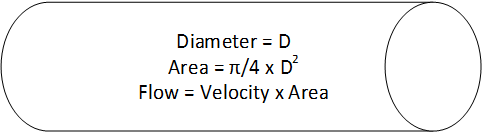
\includegraphics[scale=0.5]{PipeFlow}\\
$Q=V*A$\\
$\implies V=\dfrac{Q}{A} \implies V \Big(\dfrac{ft}{s}\Big)= \dfrac{\dfrac{10\cancel{MG}}{\cancel{day}}*\dfrac{1,000,000\cancel{gal}}{\cancel{MG}}*\dfrac{\cancelto{ft}{ft^3}}{7.48\cancel{gal}}*\dfrac{\cancel{day}}{1440*60s}}{0.785*\Big(\dfrac{24}{12}\Big)^2\cancelto{}{ft^2}}=\boxed{4.9ft/s}$

\item A wastewater flow of 3cu.ft/sec is flowing in a rectangular grit chamber.  The chamber is 2 ft 8in wide.  Wastewater is flowing 1 ft 3 in deep.  Find the velocity of the flow in this grit chamber in ft/sec.\\
\vspace{0.5cm}
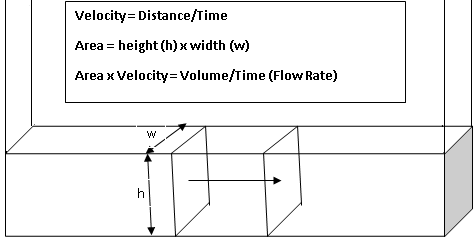
\includegraphics[scale=0.5]{ChannelFlow3}\\
$Q=V*A \implies V=\dfrac{Q}{A}$\\
$\implies V\dfrac{ft}{s}=\dfrac{3\dfrac{ft^{\cancel{3}}}{sec}}{(2 +\dfrac{8}{12})\cancel{ft} * (1+\dfrac{3}{12} \cancel{ft})}=\boxed{\dfrac{0.9ft}{sec}}$
\item How many times would the velocity increase for the same flow rate if the diameter of the pipe is reduced by half (assuming pipes are flowing full)?\\
Solution:\\
$Q=V*A \implies V=\dfrac{Q}{A}$\\
$\implies \dfrac{Velocity \enspace through \enspace the \dfrac{D}{2} \enspace pipe (V_{D/2)}}{Velocity \enspace through \enspace the \enspace D \enspace pipe (V_D)}=\dfrac{\dfrac{\cancel{Q}}{(Area of D/2 \enspace pipe)}}{\dfrac{\cancel{Q}}{(Area \enspace of \enspace D \enspace pipe)}}=\dfrac{Area \enspace of \enspace D \enspace pipe}{Area \enspace of \enspace D/2 \enspace pipe}=\dfrac{\cancel{\dfrac{\pi}{4}}\cancel{D^2}}{\cancel{\dfrac{\pi}{4}}(\dfrac{\cancel{D}}{2})^2}=\boxed{4}$
Note: $V \propto 1/A \implies V \propto 1/D^2. \enspace If \enspace D \enspace doubles,\enspace V \enspace will \enspace decrease \enspace 4X, \enspace if \enspace D \enspace triples, \enspace V \enspace will \enspace reduce \enspace 9X$

\item A flow control chamber has two channels which are each 2.5 feet wide, and 20 feet long. Only one of these channels is currently in service and it receiving a flow of 4.5 MGD. The water is flowing 1.5 feet deep in this channel. Calculate the velocity of this flow. 
Solution:\\
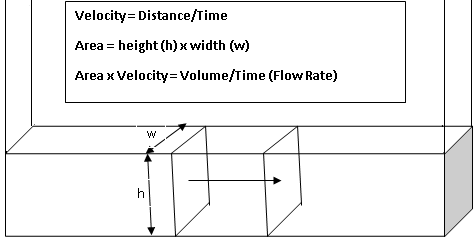
\includegraphics[scale=0.5]{ChannelFlow3}\\
$Q=V*A \implies V=\dfrac{Q}{A}$\\
$\implies V\dfrac{ft}{s}=\dfrac{4.5\dfrac{\cancel{MG}}{\cancel{day}}*\dfrac{1000000\cancel{gal}}{\cancel{MG}}*\dfrac{ft^{\cancel{3}}}{7.48\cancel{gal}}*\dfrac{\cancel{day}}{(1440*60)s}}{(2.5*1.5)\cancel{ft^2}}=\boxed{1.85\dfrac{ft}{s}}$\\

\item A wastewater channel is 3.25 feet wide and is conveying a wastewater flow of 3.5 MGD. The wastewater flow is 8 inches deep. Calculate the velocity of this flow (ft/s).\\
Solution:\\
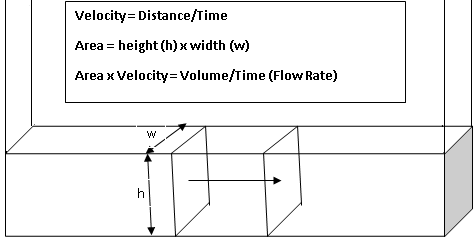
\includegraphics[scale=0.5]{ChannelFlow3}\\
$Q=V*A \implies V=\dfrac{Q}{A}$\\
$\implies V\dfrac{ft}{s}=\dfrac{3.5\dfrac{\cancel{MG}}{\cancel{day}}*\dfrac{1000000\cancel{gal}}{\cancel{MG}}*\dfrac{ft^{\cancel{3}}}{7.48\cancel{gal}}*\dfrac{\cancel{day}}{(1440*60)s}}{(3.25*\dfrac{8}{12})\cancel{ft^2}}=\boxed{2.5\dfrac{ft}{s}}$\\

\item If a chemical is added in a pipe where water is flowing at a velocity of 3.1 feet per second, how many minutes would it take for the chemical to reach a point 7 miles away?  \\

Note - we want the answer in minutes\\

$$\textrm{Min } = \dfrac{1}{3.1}\dfrac{sec}{ft}*\dfrac{5280ft}{mile}*7 miles*\dfrac{min}{60 sec} = \boxed{199 min}$$
\\

\item Find the flow in cfs in a 6 -inch line, if the velocity is 2 feet per second.

\begin{enumerate}
\item Determine the cross-sectional area of the line in square feet. Start by converting the diameter of the pipe to inches.

The diameter is 6 inches: therefore, the radius is 3 inches. 3 inches is $3 / 12$ of a foot or $0.25$ feet.

\item Now find the area in square feet.
$$
\begin{aligned}
&A=\pi \times r^{2} \\
&A=\pi \times\left(0.25 \mathrm{ft}^{2}\right. \\
&A=\pi \times 0.0625 \mathrm{ft}^{2} \\
&A=0.196 \mathrm{ft}^{2}
\end{aligned}
$$
Or
$$
\begin{aligned}
&A=0.785 \times D^{2} \\
&A=0.785 \times 0.5^{2} \\
&A=0.785 \times .05 \times .05 \\
&A=0.196 \mathrm{ft}^{2}
\end{aligned}
$$

\item Now find the flow.

$\mathrm{Q}=\mathrm{V} \times \mathrm{A}$

$\mathrm{Q}=2 \mathrm{ft} / \mathrm{sec} \times 0.196 \mathrm{ft}^{2}$

$\mathrm{Q}=0.3927 \mathrm{cfs}$ or $0.4 \mathrm{cfs}$
\end{enumerate}

\newpage
\item Calculate the velocity of a 14 MGD flow in a 6 ft wide channel with a water depth of two feet.\\
a.	7.5 ft/s\\
*b.	1.8  ft/s\\
c.	0.6 ft/s\\
d.	27 ft/s\\
e.	not enough information to solve\\
Solution:\\
\begin{center}
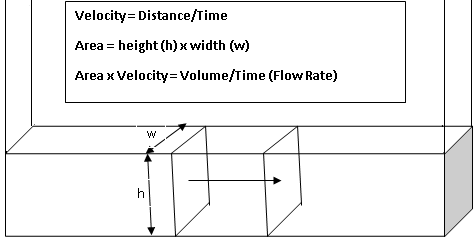
\includegraphics[scale=0.5]{ChannelFlow3}
\end{center}
$Flow (Q) = Velocity (V) * Area (A)$\\
$\implies Flow\Big[ 14 \dfrac{MG}{day}* \dfrac{10^6 gal}{MG} * \dfrac{ft^3}{7.48 gal}*\dfrac{day}{24*60*60sec}\Big]\dfrac{ft^3}{sec} = Velocity(V) \dfrac{ft}{sec}* Area (6 * 2) ft ^2$\\
\vspace{0.2cm}
$\implies 21.7 \dfrac{ft^3}{sec}= V\dfrac{ft}{sec}*12ft^2$\\
$\implies V \dfrac{ft}{sec}= \dfrac{21.7\dfrac{\cancelto{ft}{ft^3}}{sec}}{12\cancelto{}{ft^2}}= \boxed{1.8\dfrac{ft}{sec}}$\\

\item A rectangular channel 3 ft. wide contains water 2 ft. deep flowing at a velocity of 1.5 fps.
What is the flow rate in cfs?

\item Flow in an 8-inch pipe is 500 gpm. What is the average velocity in ft/sec? (Assume pipe is flowing full)

\item A pipeline is 18” in diameter and flowing at a velocity of 125 ft. per minute. What is the flow in gallons per minute?

\item The velocity in a pipeline is 2 ft./sec. and the flow is 3,000 gpm. What is the diameter of the pipe in inches?



\item Find the flow in a 4-inch pipe when the velocity is $1.5$ feet per second.


\end{enumerate}

\textbf{Solution:}\\

\begin{enumerate}

\item Solution:\\
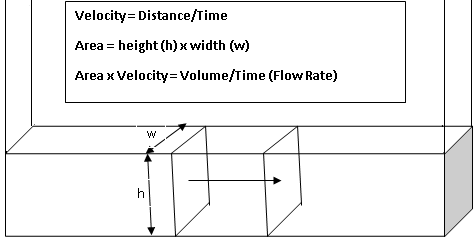
\includegraphics[scale=0.5]{ChannelFlow3}\\
$Q=V*A \implies Q = 1.5 \dfrac{ft}{sec}*(3*2)ft^2=\boxed{9\dfrac{ft^3}{sec}}$

\item Solution:\\
\vspace{0.5cm}
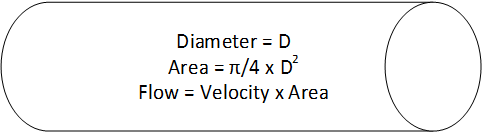
\includegraphics[scale=0.5]{PipeFlow}\\
$Q=V*A$\\
$\implies V=\dfrac{Q}{A} \implies V \Big(\dfrac{ft}{s}\Big)= \dfrac{\dfrac{500\cancel{gallon}}{\cancel{min}}*\dfrac{\cancelto{ft}{ft^3}*\dfrac{min}{60sec}}{7.48\cancel{gal}}}{0.785*\Big(\dfrac{8}{12}\Big)^2\cancelto{}{ft^2}}=\boxed{3.2ft/s}$

\item Solution:\\

\vspace{0.5cm}

The diameter of the pipe is 4 inches. Therefore, the radius is 2 inches. Convert the 2 inches to feet.
$
\begin{aligned}
&\dfrac{2}{12}=0.6667 \mathrm{ft} \\
&\mathrm{A}=\pi \times \mathrm{r}^{2} \\
&\mathrm{~A}=\pi \times(0.167 \mathrm{ft})^{2} \\
&\mathrm{~A}=\pi \times 0.028 \mathrm{ft}^{2} \\
&\mathrm{~A}=0.09 \mathrm{ft}^{2} \\
&\mathrm{Q}=\mathrm{V} \times \mathrm{A} \\
&\mathrm{Q}=1.5 \mathrm{ft} / \mathrm{sec} \times 0.09 \mathrm{ft}^{2} \\
&\mathrm{Q}=0.14 \mathrm{ft} / 3 \mathrm{sec}(\mathrm{cfs})
\end{aligned}
$



\vspace{1cm}

\item What is the velocity (ft/s) of a 3 MGD flow in a 12 in. diameter pipe. Assume the pipe is flowing full.\\

*a. 5.9 ft/s \\
b. 0.3 ft/s \\
c. 2.5 ft/s \\
d. 4 ft/s \\
\vspace{0.5cm}
Solution:\\
\vspace{0.3cm}
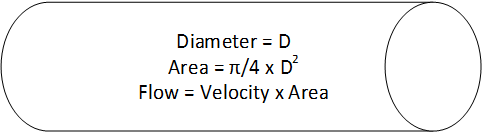
\includegraphics[scale=0.5]{PipeFlow}\\
$Q=V*A$\\
$\implies V=\dfrac{Q}{A} \implies V \Big(\dfrac{ft}{s}\Big)= \dfrac{\dfrac{3\cancel{MG}}{\cancel{day}}*\dfrac{1,000,000\cancel{gal}}{\cancel{MG}}*\dfrac{ft^{\cancel{3}}}{7.48\cancel{gal}}*\dfrac{\cancel{day}}{1440*60s}}{0.785*\Big(\dfrac{12}{12}\Big)^2\cancel{ft^2}}=\boxed{5.9 \enspace\dfrac{ft}{s}}$


\item If a chemical is added in a sewer where wastewater is flowing at a velocity of 3.1 feet per second, how many minutes would it take for the chemical to reach the plant 7 miles away?  

Note - we want the answer in minutes

Min $= \frac{1}{3.1}\frac{sec}{ft}*\frac{5280ft}{mile}*7 miles*\frac{min}{60 sec} = \boxed{199 min}$


\item A channel is 2 feet 4 inches wide. When water is flowing 8 inches deep in this channel, the flow is found to be 1.6 ft per second. Calculate flow in MGD.\\
\vspace{0.3cm}
Solution:\\
\vspace{0.3cm}
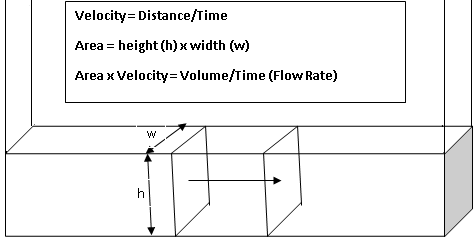
\includegraphics[scale=0.5]{ChannelFlow3}\\
$Q=V*A$\\
$Q=1.6\dfrac{ft}{s}*\Big(\dfrac{28}{12}*\dfrac{8}{12}\Big)ft^2=2.49\dfrac{ft^3}{s}$\\
$Q=2.49\dfrac{\cancel{ft^3}}{\cancel{s}}*\dfrac{(1440*60)\cancel{s}}{day}*7.48\dfrac{\cancel{gal}}{\cancel{ft^3}}\dfrac{MG}{\cancel{gal}}=\boxed{1.61MGD}$


\item A transmission line to a water treatment plant is 12 miles long. If the water is flowing at 2.2 fps, approximately.  How long will it take for wastewater to reach the plant?\\
Solution:\\
$time \enspace to \enspace reach \enspace plant \enspace (hrs)=\dfrac{\cancel{s}}{2.2\cancel{ft}}*\dfrac{5280\cancel{ft}}{\cancel{mile}}*12\cancel{miles}*\dfrac{hrs}{(60*60)\cancel{s}}=\boxed{8hrs}$ 


\item A water main feeds a subdivision. The main is 500 feet long and 12-inches in diameter. The pipe delivers an average flow of $30 \mathrm{cfm}$. The distribution crew is flushing the main to remove sediment. How long should they flush the line to achieve 2 pipe volumes?\\
\vspace{0.3cm}
$\textrm{time}=\dfrac{\textrm{flush \enspace volume}}{\textrm{flow \enspace rate} - \dfrac{\textrm{volume}}{\textrm{time}}}=\dfrac{2 * \Big(0.785*\Big(\dfrac{12}{12}\Big)^2 \enspace \textrm{ft}^2 *500 \enspace \textrm{ft}\Big)\cancel{\textrm{ft}^3}}{\dfrac{30 \enspace \cancel{\mathrm{ft}^3}}{\textrm{min}}}=\boxed{26 \enspace \textrm{min}} $
\vspace{0.3cm}

\item Flow in an 8-inch pipe is 500 gpm. What is the average velocity in ft/sec? (Assume pipe is flowing full)\\
Solution:\\
\vspace{0.2cm}

$Flow \enspace(\mathrm{Q})= Velocity \enspace(\mathrm{V})  \times Area \enspace(\mathrm{A}) \implies Q=V*A \implies V=\dfrac{Q}{A}$\\
We need to convert Q which is given in gpm to ft${^3}$/sec and calculate the area of the pipe in ft${^2}$ so velocity can be valculated in ft/sec.\\
\vspace{0.2cm}
$ V \dfrac{ft}{sec} = \dfrac{Q \enspace \dfrac{\cancelto{ft}{ft^3}}{sec}}{A \enspace\cancel{ft}}$\\
\vspace{0.2cm}
Step 1 - Converting Q - 500 gpm to ft${^3}/min$:\\
\vspace{0.2cm}
$\dfrac{500 \enspace \cancel{gallons}}{\bcancel{min}}*\dfrac{ft^3}{7.48 \enspace \cancel{gallon}}*\dfrac{\bcancel{min}}{60 \enspace sec}=1.1\dfrac{ft^3}{sec}$\\
\vspace{0.2cm}
Step 2 - Calculating area in ft${^2}$:\\
\vspace{0.2cm}
$Area \enspace ft^2= \dfrac{\pi}{4}*D^2= 0.785*\Big(\dfrac{8}{12}\Big)^2 \enspace ft^2=0.785*\dfrac{64}{144}=1.766 \enspace ft^2$\\
\vspace{0.2cm}
$\implies V \dfrac{ft}{sec} = \dfrac{ 1.1 ft^3/sec}{0.349 \enspace ft^2} = \boxed{3.2 ft/sec}$\\
\vspace{0.3cm} 


\item A pipeline is 18” in diameter and flowing at a velocity of 125 ft. per minute. What is the flow in gallons per minute?\\
\vspace{0.2cm}
Solution:\\
$Flow \enspace(\mathrm{Q}) \enspace = Velocity \enspace(\mathrm{V})  \times Area \enspace(\mathrm{A})$\\
\vspace{0.2cm}
As the velocity is given in ft/min, and the area can be calculated in ft$^2$, flow can be calulated in ft$^3$/min and then converted to gal/min.\\
\vspace{0.2cm}

\vspace{0.2cm}
Step 1:  Calculating area in ft${^2}$:\\
\vspace{0.2cm}
$Area \enspace (ft^2)= \dfrac{\pi}{4}*D^2= 0.785*\Big(\dfrac{18}{12}\Big)^2 \enspace ft^2=0.785*\dfrac{324}{144}=0.349 \enspace ft^2$\\
\vspace{0.2cm}

Step 2: Calculate flow in ft$^3$/min:\\

$ Q \enspace ft^3/min = 125 \dfrac{ft}{min}*1.77 \enspace ft^2 = 221.25 \dfrac{ft^3}{min}$\\

\vspace{0.2cm}

Step 3: Convert Q to gallons per minute

\vspace{0.2cm}

$Q=221.25 \dfrac{\cancel{ft^3}}{min}*7.48\dfrac{gal}{\cancel{ft^3}}=\boxed{1655 \dfrac{gal}{min}}$


\item The velocity in a pipeline is 2 ft./sec. and the flow is 3,000 gpm. What is the diameter of the pipe in inches?

Solution:\\
\vspace{0.2cm}

$Flow \enspace(\mathrm{Q})= Velocity \enspace(\mathrm{V})  \times Area \enspace(\mathrm{A}) \implies Q=V*A \implies A=\dfrac{Q}{V}$\\
We need to convert Q which is given in gpm to ft${^3}$/sec and calculate the area of the pipe in ft${^2}$ given the velocity.\\
From the calculated area of the pipe, the pipe diameter can be calculated.\\
\vspace{0.2cm}
$ A \dfrac{ft}{sec} = \dfrac{Q \enspace \dfrac{\cancelto{ft^2}{ft^3}}{\cancel{sec}}}{V \enspace \dfrac{\cancelto{}{ft}}{\cancel{sec}}}$\\
\vspace{0.2cm}
Step 1 - Converting Q - 3000 gpm to ft${^3}$/sec:\\
\vspace{0.2cm}
$\dfrac{3000 \enspace \cancel{gallons}}{\bcancel{min}}*\dfrac{ft^3}{7.48 \enspace \cancel{gallon}}*\dfrac{\bcancel{min}}{60 \enspace sec}=6.68\dfrac{ft^3}{sec}$\\
\vspace{0.2cm}
Step 2 - Calculating area in ft${^2}$:\\
\vspace{0.2cm}
$\implies A \enspace ft^2 = \dfrac{ 6.68 ft^3/sec}{2 \dfrac{ft}{sec}} = 3.34 ft^2$\\
\vspace{0.3cm} 
$Area \enspace (A)= \dfrac{\pi}{4}*D^2 = 0.785*D^2 \implies D^2=\dfrac{A}{0.785} \implies D=\Big(\dfrac{A }{0.785}\Big)^{\dfrac{1}{2}}$\\
$\implies D=\Big(\dfrac{3.34}{0.785}\Big)^{\dfrac{1}{2}}=\boxed{2 \enspace ft}$\\
\vspace{0.2cm}

\item Find the flow in a 4-inch pipe when the velocity is $1.5$ feet per second.

Solution:\\
$Flow \enspace(\mathrm{Q}) \enspace = Velocity \enspace(\mathrm{V})  \times Area \enspace(\mathrm{A})$\\
\vspace{0.2cm}
The velocity is given in ft/sec and after calculating the area in ft$^2$, flow can be calulated in ft$^3$/min.\\
\vspace{0.2cm}

\vspace{0.2cm}
Step 1:  Calculating area in ft${^2}$:\\
\vspace{0.2cm}
$Area \enspace (ft^2)= \dfrac{\pi}{4}*D^2= 0.785*\Big(\dfrac{4}{12}\Big)^2 \enspace ft^2=0.785*\dfrac{324}{144}=0.087 \enspace ft^2$\\
\vspace{0.2cm}

Step 2: Calculate flow in ft$^3$/min:\\

$ Q \enspace ft^3/min = 1.5 \dfrac{ft}{sec}*0.087 \enspace ft^2 = 0.13 \dfrac{ft^3}{sec}$\\

\vspace{0.2cm}

Q can be converted to a more commonly used gallons per minute unit

\vspace{0.2cm}

$Q=0.13 \dfrac{\cancel{ft^3}}{sec}*7.48\dfrac{gal}{\cancel{ft^3}}*60\dfrac{sec}{\cancel{min}}=\boxed{59 \dfrac{gal}{min}}$
  \item A 42-inch diameter pipe transfers 35 cubic feet of water per second. Find the velocity in $\mathrm{ft} / \mathrm{sec}$. 

  Solution:\\
\vspace{0.2cm}

$Flow \enspace(\mathrm{Q})= Velocity \enspace(\mathrm{V})  \times Area \enspace(\mathrm{A}) \implies Q=V*A \implies V=\dfrac{Q}{A}$\\
Q is already given in ft${^3}$/sec.  We need to first calculate the area of the pipe in ft${^2}$ so velocity can be valculated in ft/sec.\\
\vspace{0.2cm}
$ V \dfrac{ft}{sec} = \dfrac{Q \enspace \dfrac{\cancelto{ft}{ft^3}}{sec}}{A \enspace\cancel{ft}}$\\
\vspace{0.2cm}
Step 1 - Calculating area in ft${^2}$:\\
\vspace{0.2cm}
$Area \enspace ft^2= \dfrac{\pi}{4}*D^2= 0.785*\Big(\dfrac{42}{12}\Big)^2 \enspace ft^2=0.785*\dfrac{1764}{144}=9.616 \enspace ft^2$\\
\vspace{0.2cm}
$\implies V \dfrac{ft}{sec} = \dfrac{ 35 ft^3/sec}{9.616 \enspace ft^2} = \boxed{3.6 ft/sec}$\\
\vspace{0.3cm} 

  
  \item A plastic float is dropped into a channel and is found to travel 10 feet in $4.2$ seconds. The channel is $2.4$ feet wide and the water is flowing $1.8$ feet deep. Calculate the flow rate of water in cfs.\\
  \vspace{0.2cm}
  Solution:\\
  $Flow \enspace(\mathrm{Q})= Velocity \enspace(\mathrm{V})  \times Area \enspace(\mathrm{A})$\\

The speed of the float travelling is the velocity of the water $\implies Velocity = \dfrac{10 \enspace ft}{4.2 \enspace sec}$

Thus flow = $\dfrac{10 \enspace ft}{4.2 \enspace sec} * (2.4*1.8) ft^2 = \boxed{4.32 \dfrac{ft^3}{sec}} $\\

\vspace{0.2cm}

\end{enumerate}



\end{document}